%%%%%%%%%%%%%%%%%%%%%%%%%%%%%%%%%%%%%%%%%
% Dreuw & Deselaer's Poster
% LaTeX Template
% Version 1.0 (11/04/13)
%
% Created by:
% Philippe Dreuw and Thomas Deselaers
% http://www-i6.informatik.rwth-aachen.de/~dreuw/latexbeamerposter.php
%
% This template has been downloaded from:
% http://www.LaTeXTemplates.com
%
% Edited by: Manfred Brill
%
% License:
% CC BY-NC-SA 3.0 (http://creativecommons.org/licenses/by-nc-sa/3.0/)
%%%%%%%%%%%%%%%%%%%%%%%%%%%%%%%%%%%%%%%%%

% ----------------------------------------------------------------------------------------
%  Kopf- und Fusszeile werden in beamertheme16pd2.sty definiert!
% ----------------------------------------------------------------------------------------

%----------------------------------------------------------------------------------------
%   PACKAGES AND OTHER DOCUMENT CONFIGURATIONS
%----------------------------------------------------------------------------------------
\documentclass[final,hyperref={pdfpagelabels=false}]{beamer}

\usepackage{todo}

\usepackage{wrapfig}

\usepackage[orientation=portrait, size=a0, scale=1.4]{beamerposter}

\usetheme{I6pd2} % Use the I6pd2 theme supplied with this template

\usepackage[german]{babel}
%\usepackage[english]{babel} % English language/hyphenation

\usepackage{amsmath,amsthm,amssymb,latexsym}

%\usepackage{times}\usefonttheme{professionalfonts}  % Uncomment to use Times as the main font
%\usefonttheme[onlymath]{serif} % Uncomment to use a Serif font within math environments

\boldmath % Use bold for everything within the math environment

\usepackage{booktabs} % Top and bottom rules for tables

\usepackage{multicol}

\usepackage{url}

\usepackage{bibgerm}

\usepackage{hyperref}

\usepackage[misc]{ifsym}

\usepackage{enumitem}

\newcommand{\imagePath}{./figures}

\graphicspath{{figures/}} % Location of the graphics files

\usecaptiontemplate{\small\structure{\insertcaptionname~\insertcaptionnumber: }\insertcaption}
 % A fix for figure numbering

%----------------------------------------------------------------------------------------
%   TITLE SECTION
%----------------------------------------------------------------------------------------



\title{\huge DICOM StereoViewer}

\author{Rafael Hoock}

\institute{Fachbereich Informatik und Mikrosystemtechnik}
%----------------------------------------------------------------------------------------

\begin{document}

\addtobeamertemplate{block end}{}{\vspace*{2ex}} % White space under blocks

\begin{frame}[t] % The whole poster is enclosed in one beamer frame



%\vspace{0.125cm}

% ---

\begin{columns}[t] % The whole poster consists of two major columns, each of which can be subdivided further with another \begin{columns} block - the [t] argument aligns each column's content to the top

\begin{column}{.025\textwidth}\end{column} % Empty spacer column

\begin{column}{.465\textwidth} % The first column


\begin{block}{Workflow}

    \begin{figure}
        \centering
        % 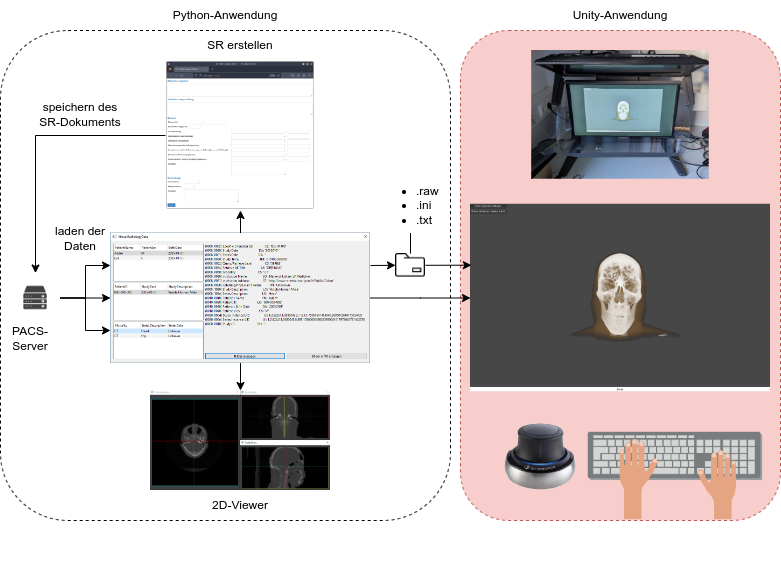
\includegraphics[width=0.76\textwidth]{workflow}
        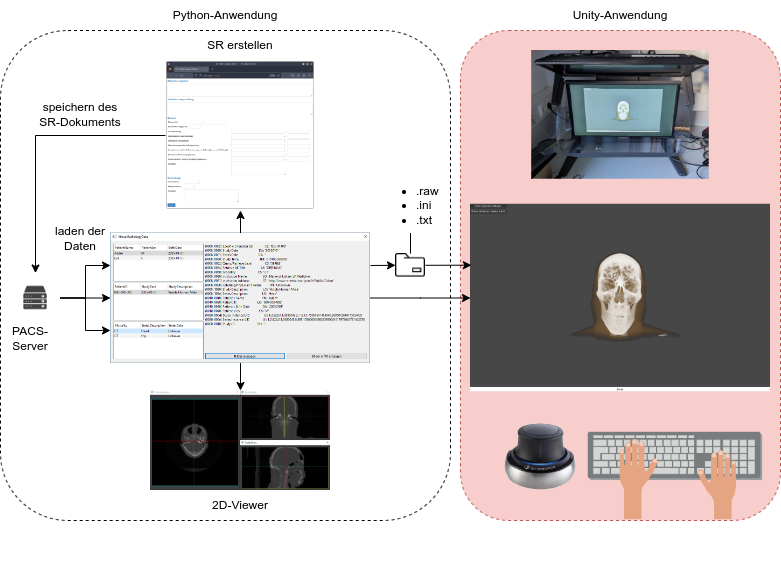
\includegraphics[height=21cm]{workflow}
    \end{figure}
%
%\begin{itemize}
% \item In der Applikation werden vorberechnete Kurvendaten importiert und im Raum dargestellt. Anhand einer Initialisierungsdatei wird die Szene f"ur eine Lerneinheit individuell angepasst, indem Elemente im Raum de- bzw. aktiviert werden.    
% \item Auf einem Tisch wird die Kurve in reduziert skalierter Form dargestellt. Mit Buttons kann durch den Datensatz von Kurven navigiert werden. Aus welcher Sicht eine Kurve betrachtet wird, kann ebenfalls hierdurch gesteuert werden.  %können weitere Kurven zur Darstellung ausgewählt werden.
% \item Flugzeuge fliegen durch Benutzeraktion entlang der Kurve und visualisieren den Weg der Kurve. Verschiedene Flugzeuge visualisieren unterschiedliche Parametrisierungen der Kurve  %Der Benutzer kann den Raytracing-Prozess durch Betätigen von Buttons in der Szene steuern und verfolgen.
% 
%    \end{itemize}
    
    %\vspace{20px}
\end{block}

\end{column}

% -------

\begin{column}{.025\textwidth}\end{column} % Empty spacer column

\begin{column}{0.465\textwidth}

\begin{block}{Verwaltung von Patientendaten}

    \begin{figure}
        \centering
        
        % 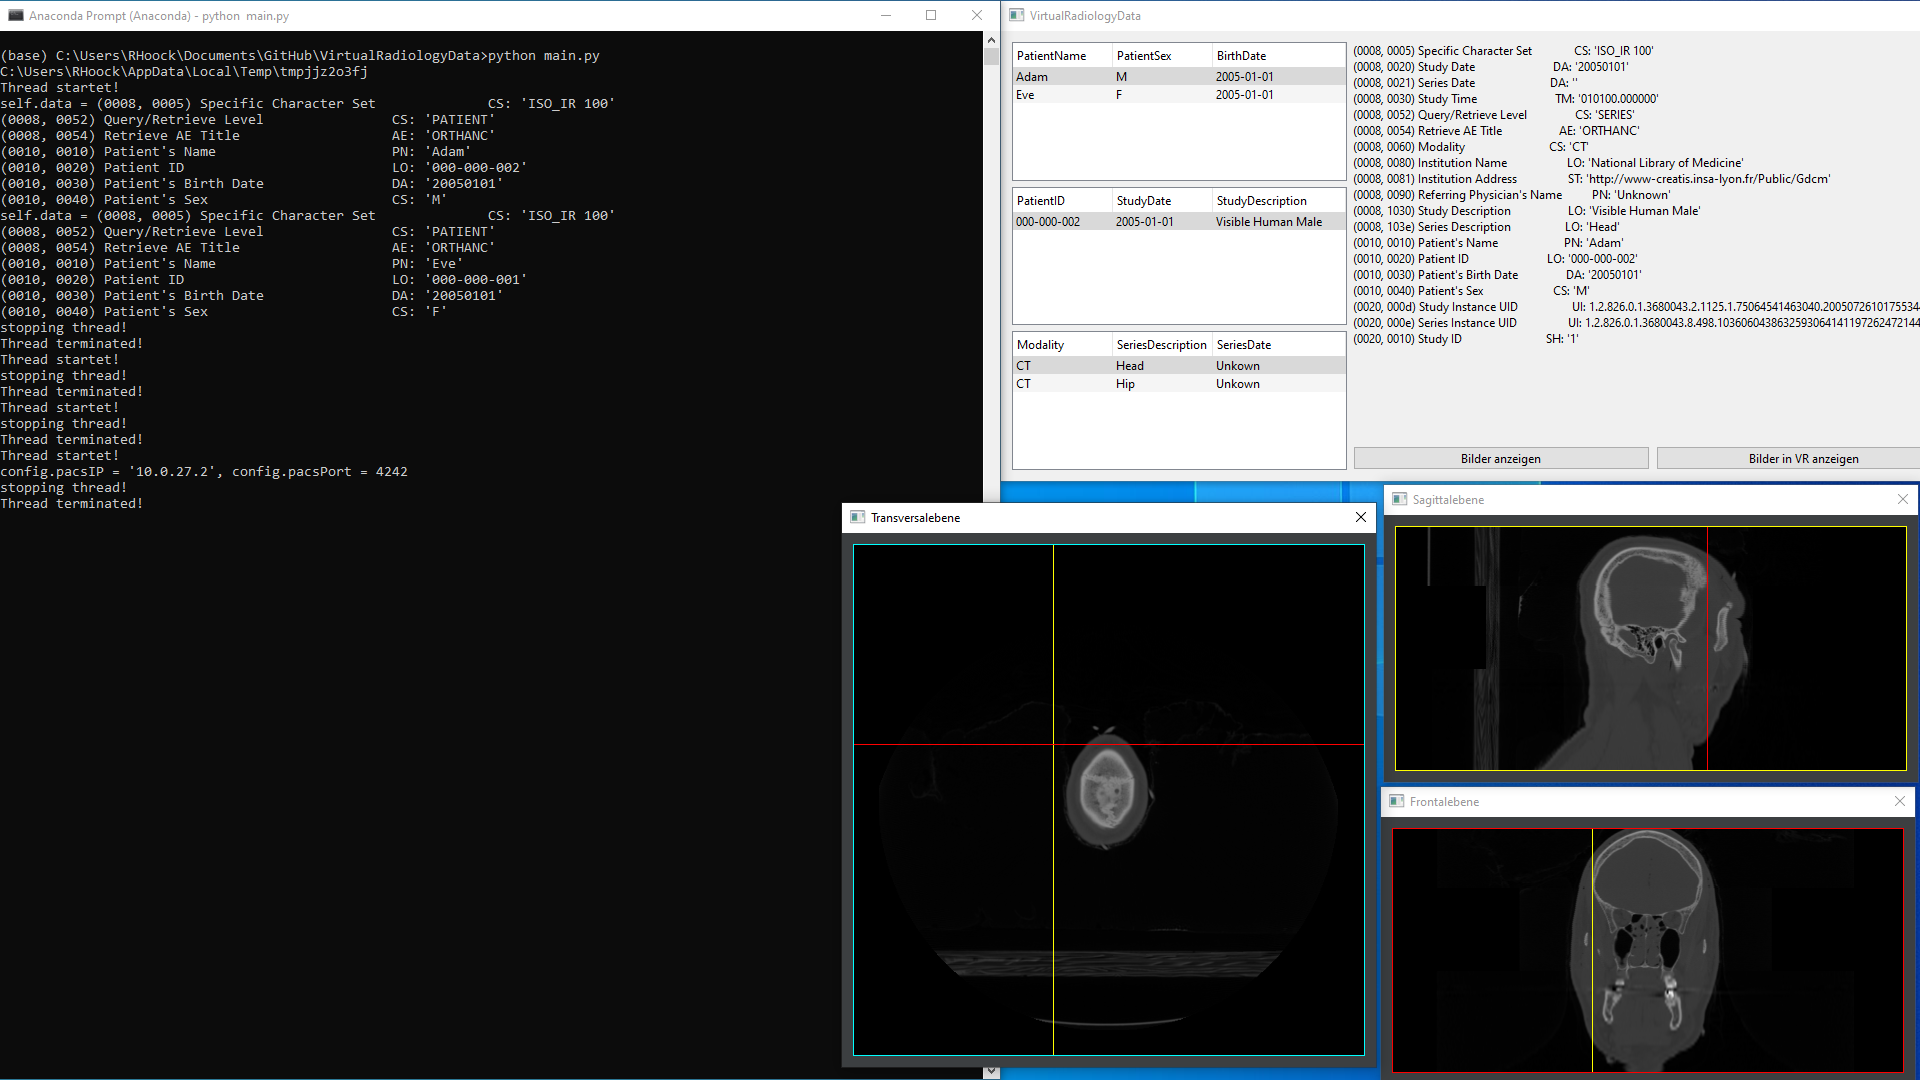
\includegraphics[width=1.0\textwidth]{pythonApplication01}
        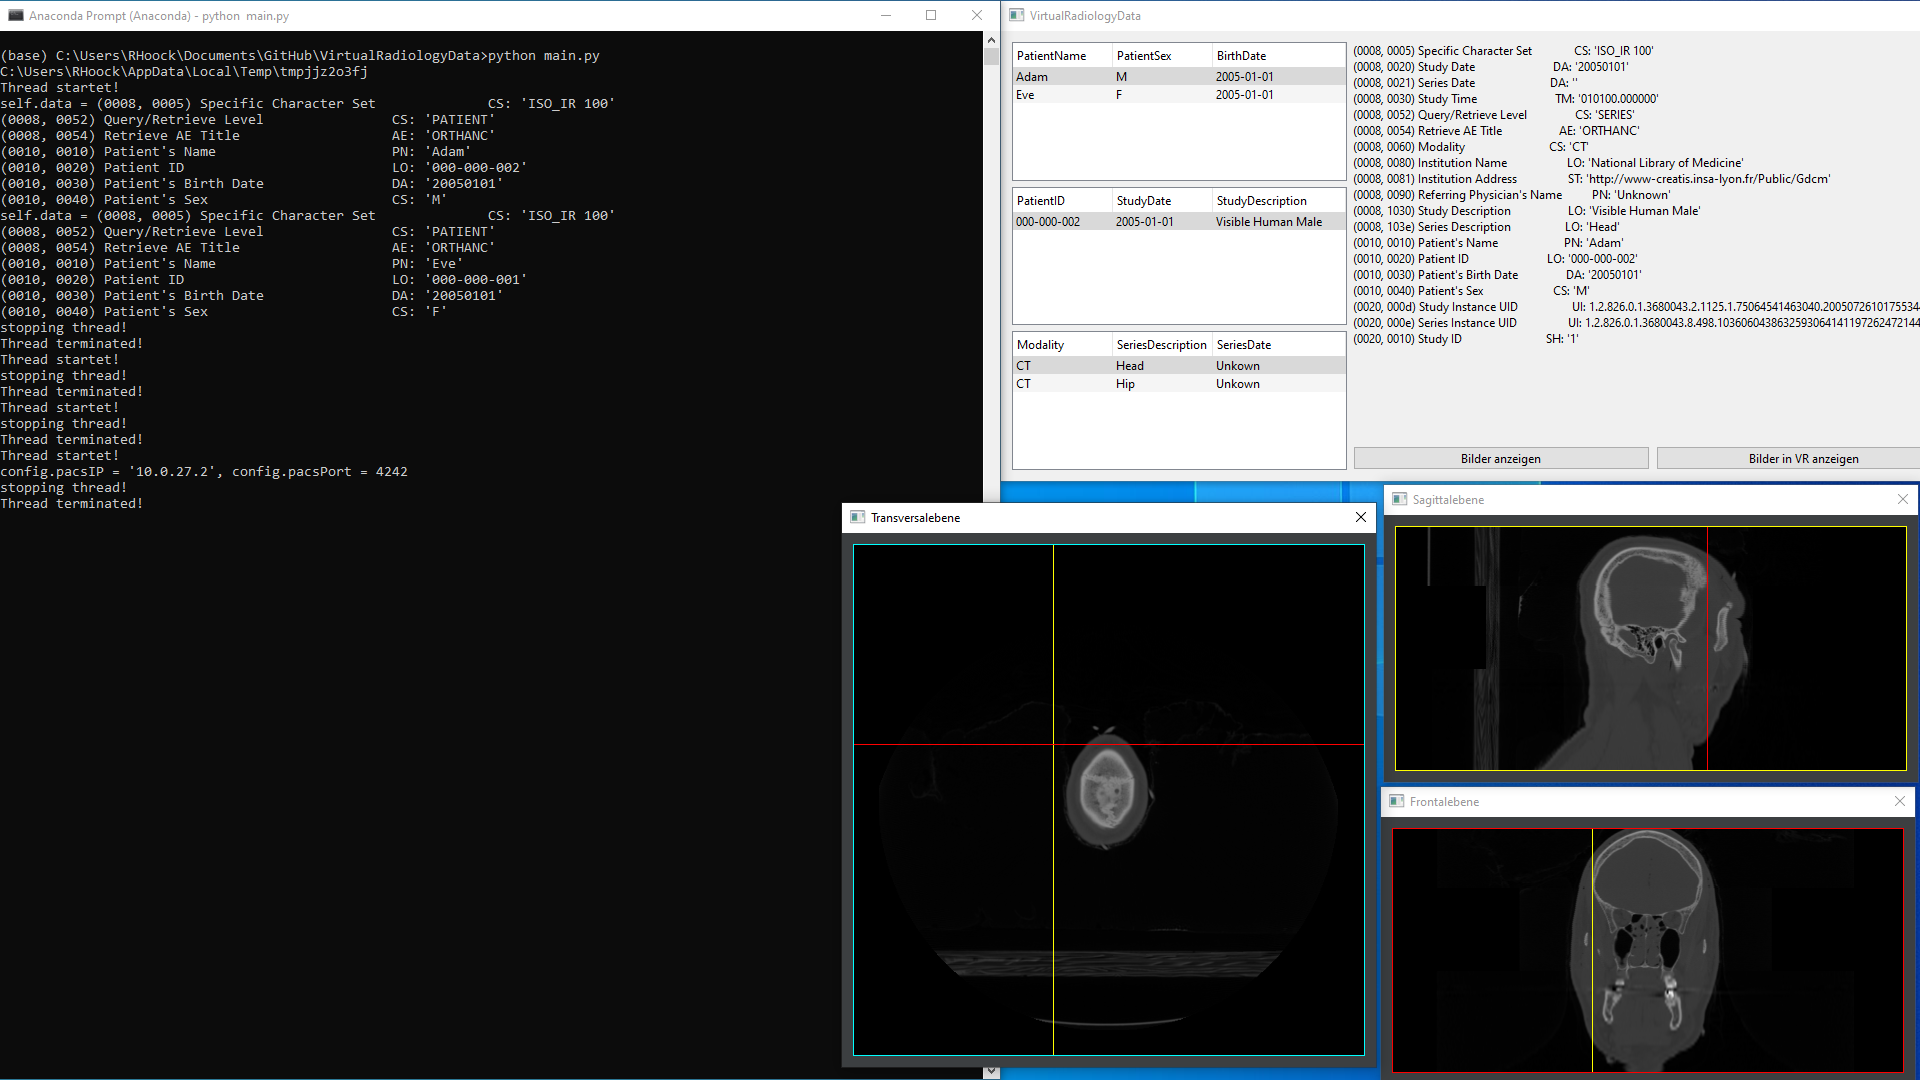
\includegraphics[height=21cm]{pythonApplication01}
    \end{figure}
%
%\begin{itemize}
% \item In der Applikation werden vorberechnete Kurvendaten importiert und im Raum dargestellt. Anhand einer Initialisierungsdatei wird die Szene f"ur eine Lerneinheit individuell angepasst, indem Elemente im Raum de- bzw. aktiviert werden.    
% \item Auf einem Tisch wird die Kurve in reduziert skalierter Form dargestellt. Mit Buttons kann durch den Datensatz von Kurven navigiert werden. Aus welcher Sicht eine Kurve betrachtet wird, kann ebenfalls hierdurch gesteuert werden.  %können weitere Kurven zur Darstellung ausgewählt werden.
% \item Flugzeuge fliegen durch Benutzeraktion entlang der Kurve und visualisieren den Weg der Kurve. Verschiedene Flugzeuge visualisieren unterschiedliche Parametrisierungen der Kurve  %Der Benutzer kann den Raytracing-Prozess durch Betätigen von Buttons in der Szene steuern und verfolgen.
% 
%    \end{itemize}
    
    %\vspace{20px}
\end{block}


\end{column}

\begin{column}{.025\textwidth}\end{column} % Empty spacer column

\end{columns} % End of all the columns in the poster


\begin{columns}[t] % The whole poster consists of two major columns, each of which can be subdivided further with another \begin{columns} block - the [t] argument aligns each column's content to the top

\begin{column}{.025\textwidth}\end{column} % Empty spacer column

\begin{column}{.465\textwidth} % The first column

\begin{block}{Technologien}
   \begin{figure}
       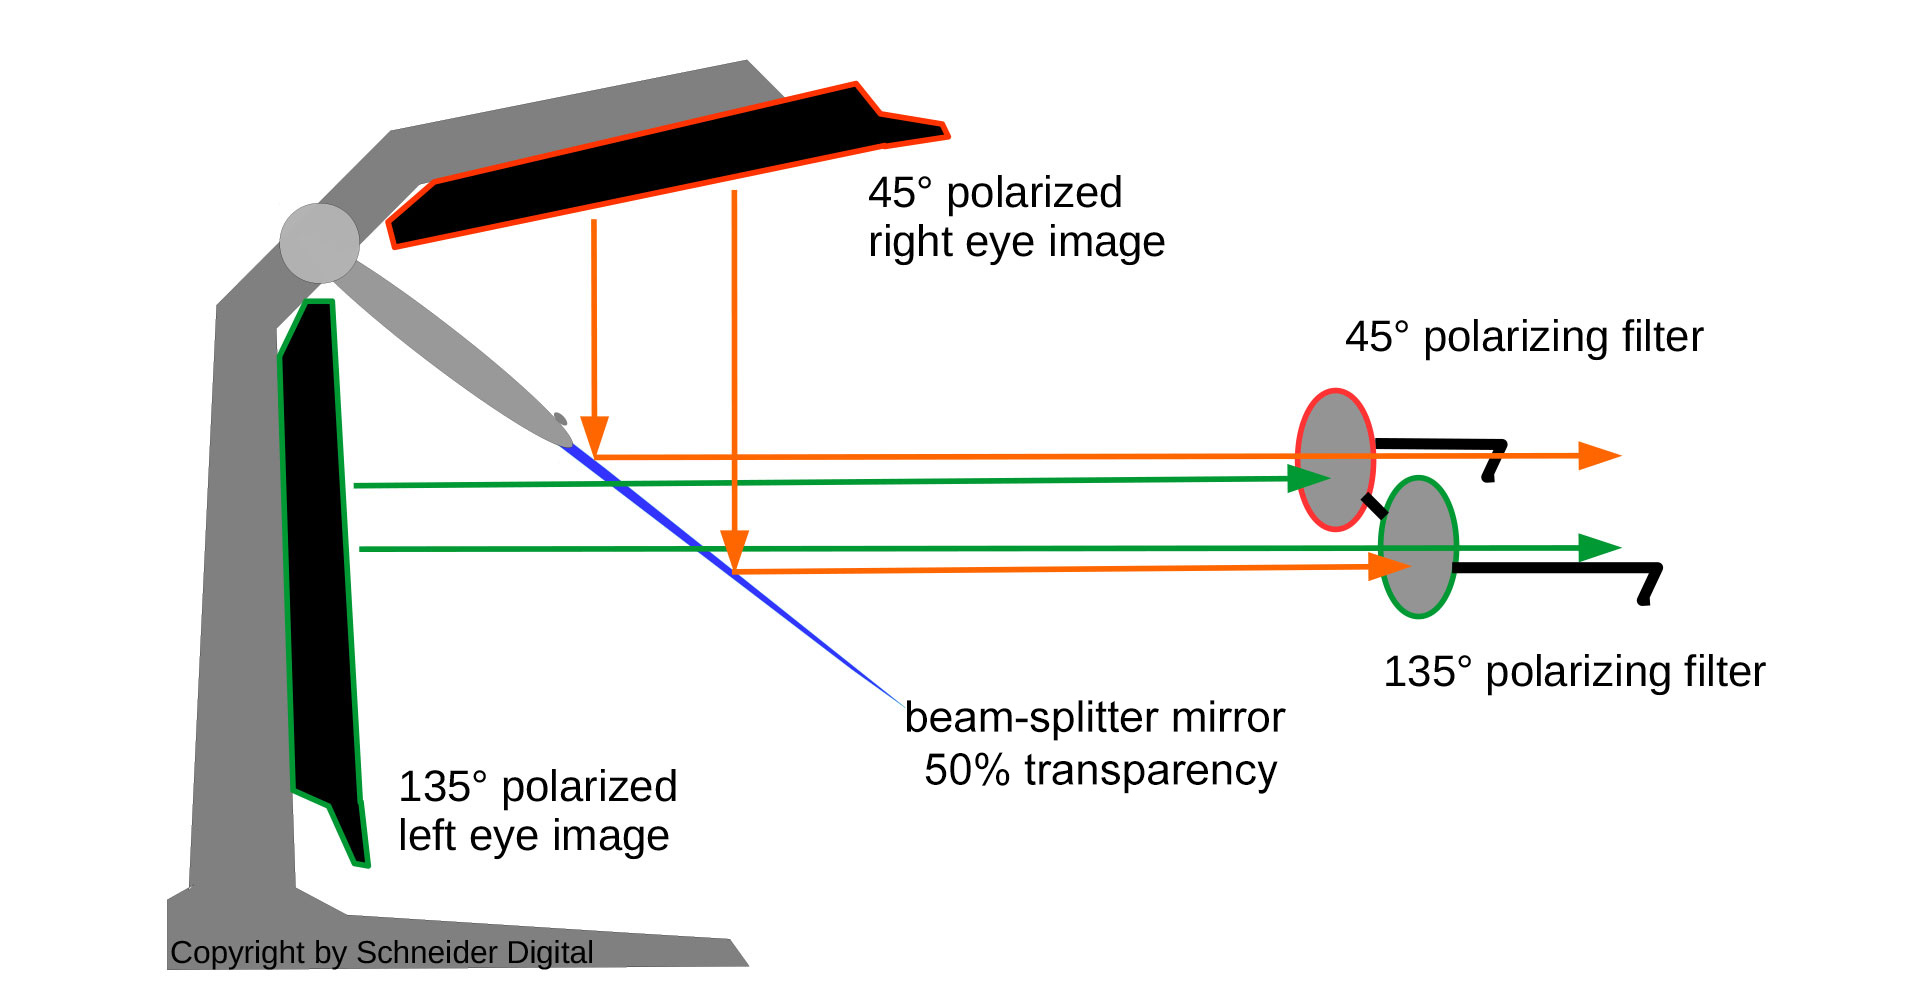
\includegraphics[height=12cm]{pluraviewTechnologie}
       \includegraphics[height=12cm]{spacenagivator\_dof}
   	 % \includegraphics[height=14.25cm]{hmd}\hspace*{0.25cm}
       %\includegraphics[height=14.25cm]{dxrWorkspace}
   	 % \includegraphics[height=14.25cm]{hmdSmall}
   	%\includegraphics[height=14.25cm]{caveSlim}
   \end{figure}
   
%   \begin{itemize}
%   \item Unter dem Sammelbegriff \textbf{Cross-Reality (XR)} werden Techniken der digitalen Konstruktion und Unterst\"utzung von Realit\"aten zusammengefasst.
%   \item Applikationen dieser Art finden vermehrt Einsatz in Industrie, Unterhaltung und Lehre.
%   \item Im \textbf{Virtual und Augmented Reality Lab} der Hochschule Kaiserslautern werden Prototypen konzeptioniert und entwickelt, um die Lehre an der Hochschule besser unterst\"utzen zu k\"onnen.
%   \end{itemize}
   
     
   
   
\end{block}


\vspace{0.125cm}

\end{column}

% -------

\begin{column}{.025\textwidth}\end{column} % Empty spacer column

\begin{column}{0.465\textwidth}

\begin{block}{PluraView + Polfilterbrille}
   \begin{figure}
       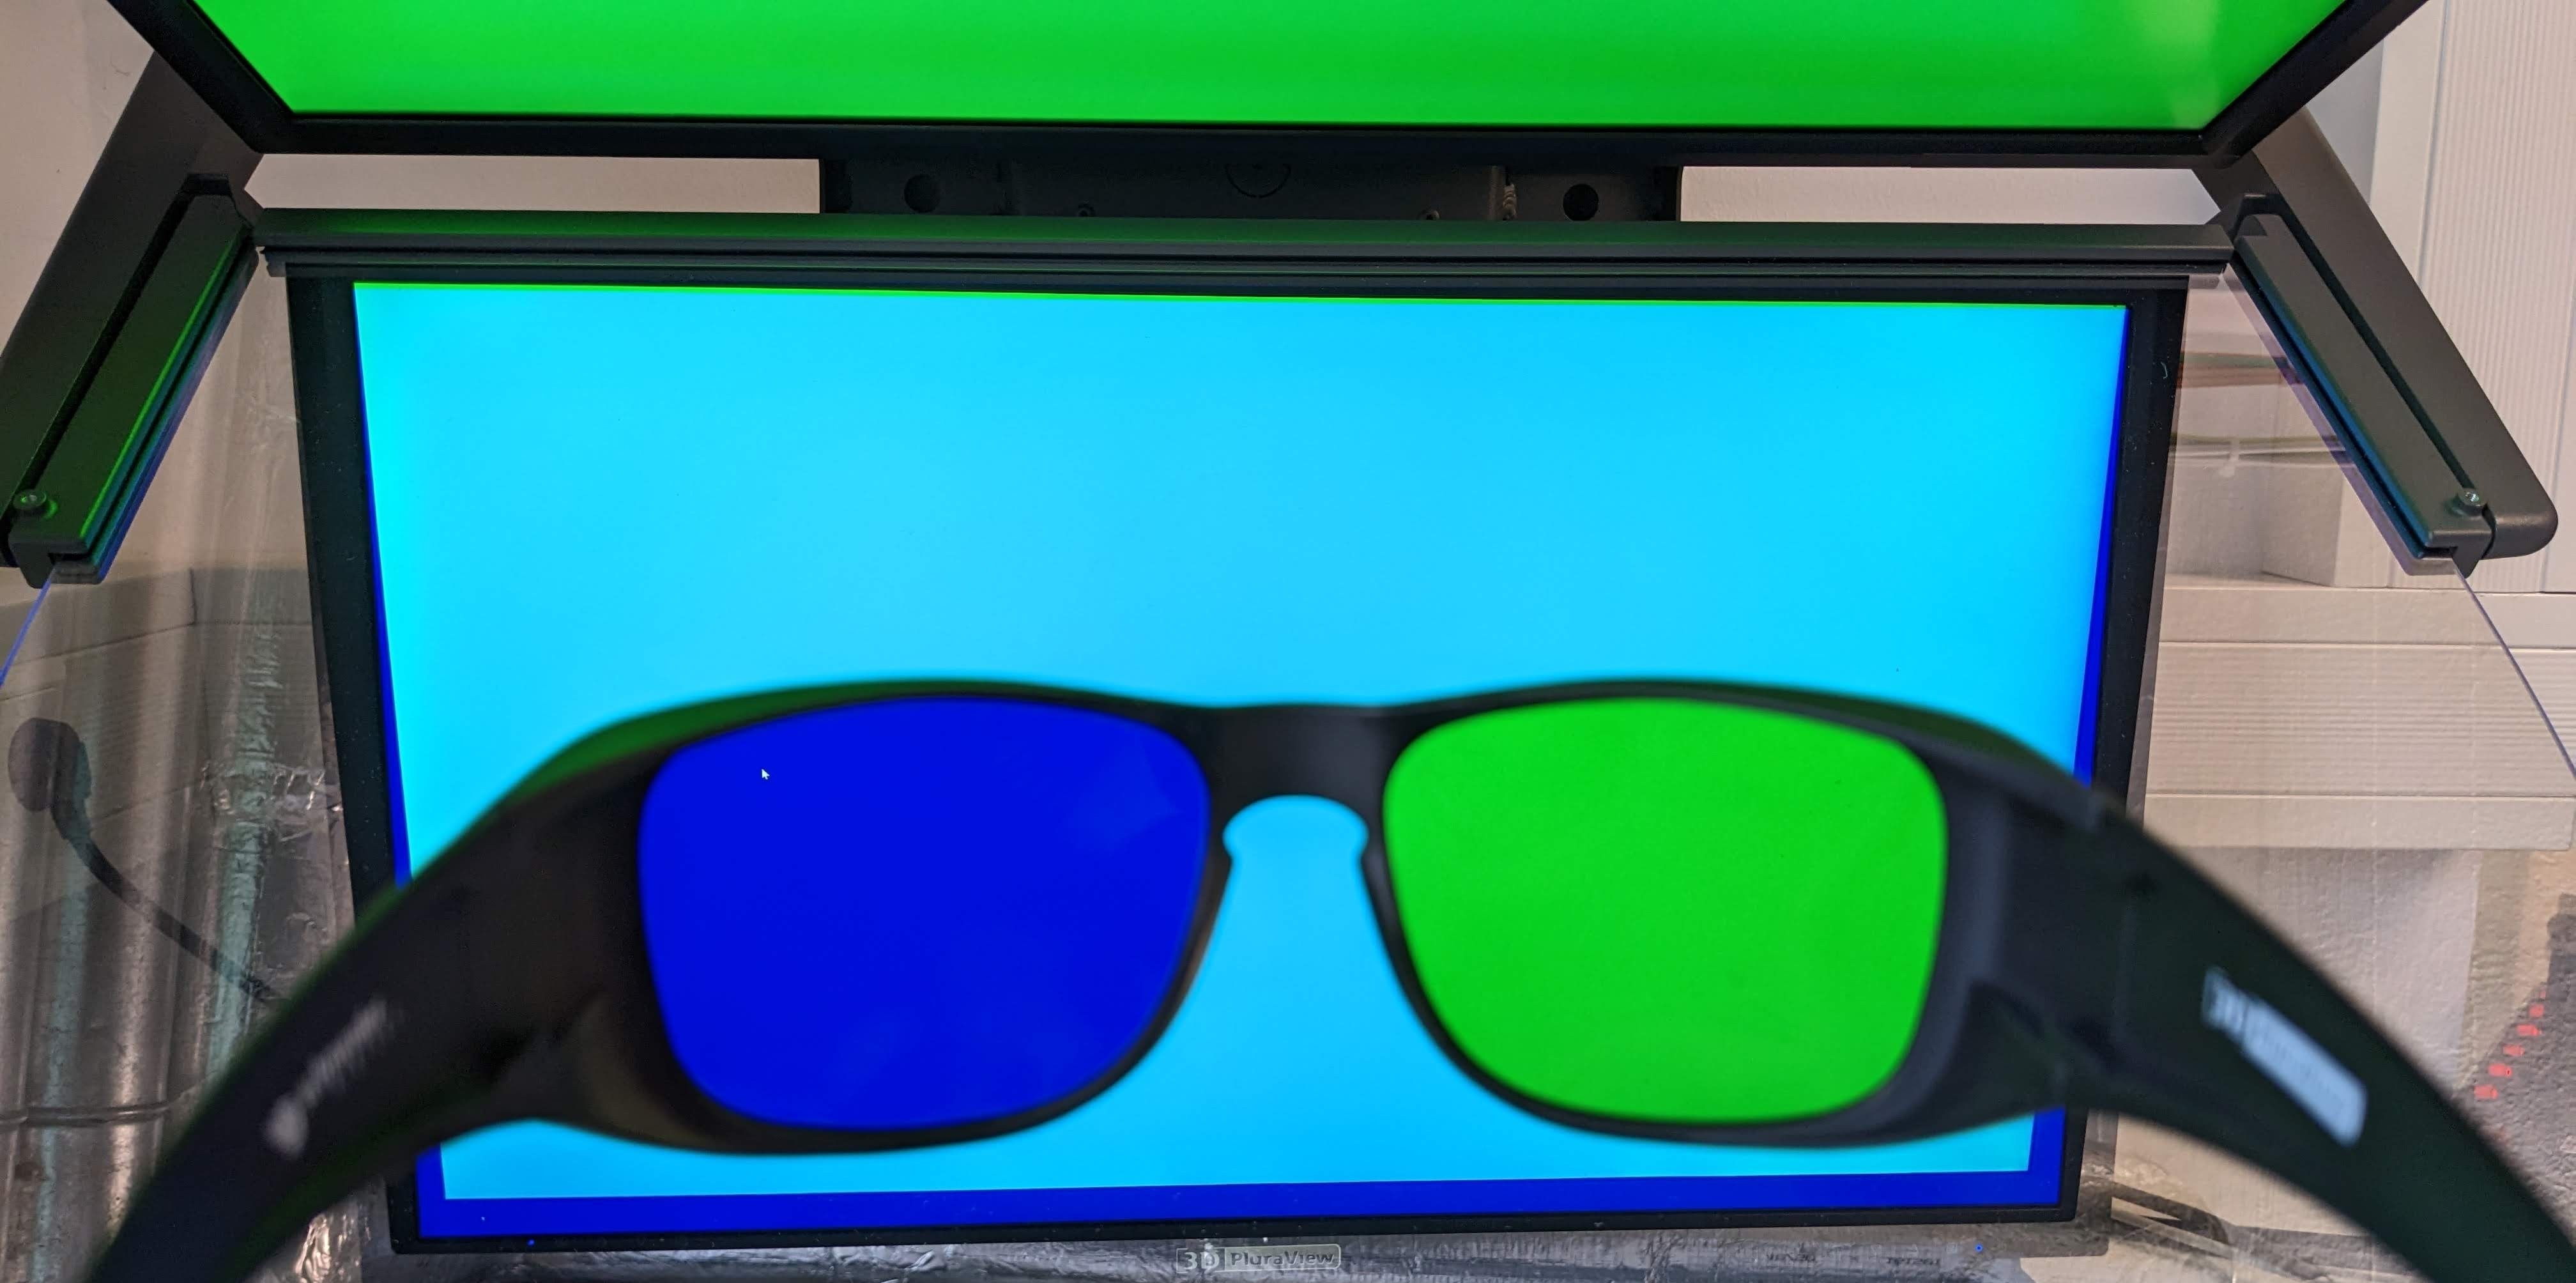
\includegraphics[height=12cm]{pluraviewBrille}
   \end{figure}
    %\vspace{140px}
    %\begin{figure}
    %	\center
        %\includegraphics[width=0.475\linewidth]{lemniskate_gerono}\hspace*{0.25cm}
        %\includegraphics[width=0.475\linewidth]{helix}
        %\caption{Visualisierung eines Raytracing-Vorgangs \cite{Suffern}}
    %\end{figure}
    
    %\vspace{120px}

%	\begin{itemize}
		%\item Darstellung von Parameterkurven
	 	%\item Standardthema in Vorlesungen der computergestützten Mathematik 
	 	%\item \textbf{Problem:} \\ Raumkurven schwer für Lernende verständlich darstellbar
	 	%\item \textbf{Idee:} \\ Visualisieren der Raumkurven in einer Virtual Reality Umgebung
	%\end{itemize}

%\vspace{1cm}

\end{block}



\end{column} % End of the second column



\begin{column}{.025\textwidth}\end{column} % Empty spacer column

\end{columns} % End of all the columns in the poster

\begin{columns}[t] % The whole poster consists of two major columns, each of which can be subdivided further with another \begin{columns} block - the [t] argument aligns each column's content to the top

\begin{column}{.025\textwidth}\end{column} % Empty spacer column

\begin{column}{.465\textwidth} % The first column


\begin{block}{Kopf + Transferfunktion}
%    %\vspace{140px}
    \begin{figure}
    	\center
        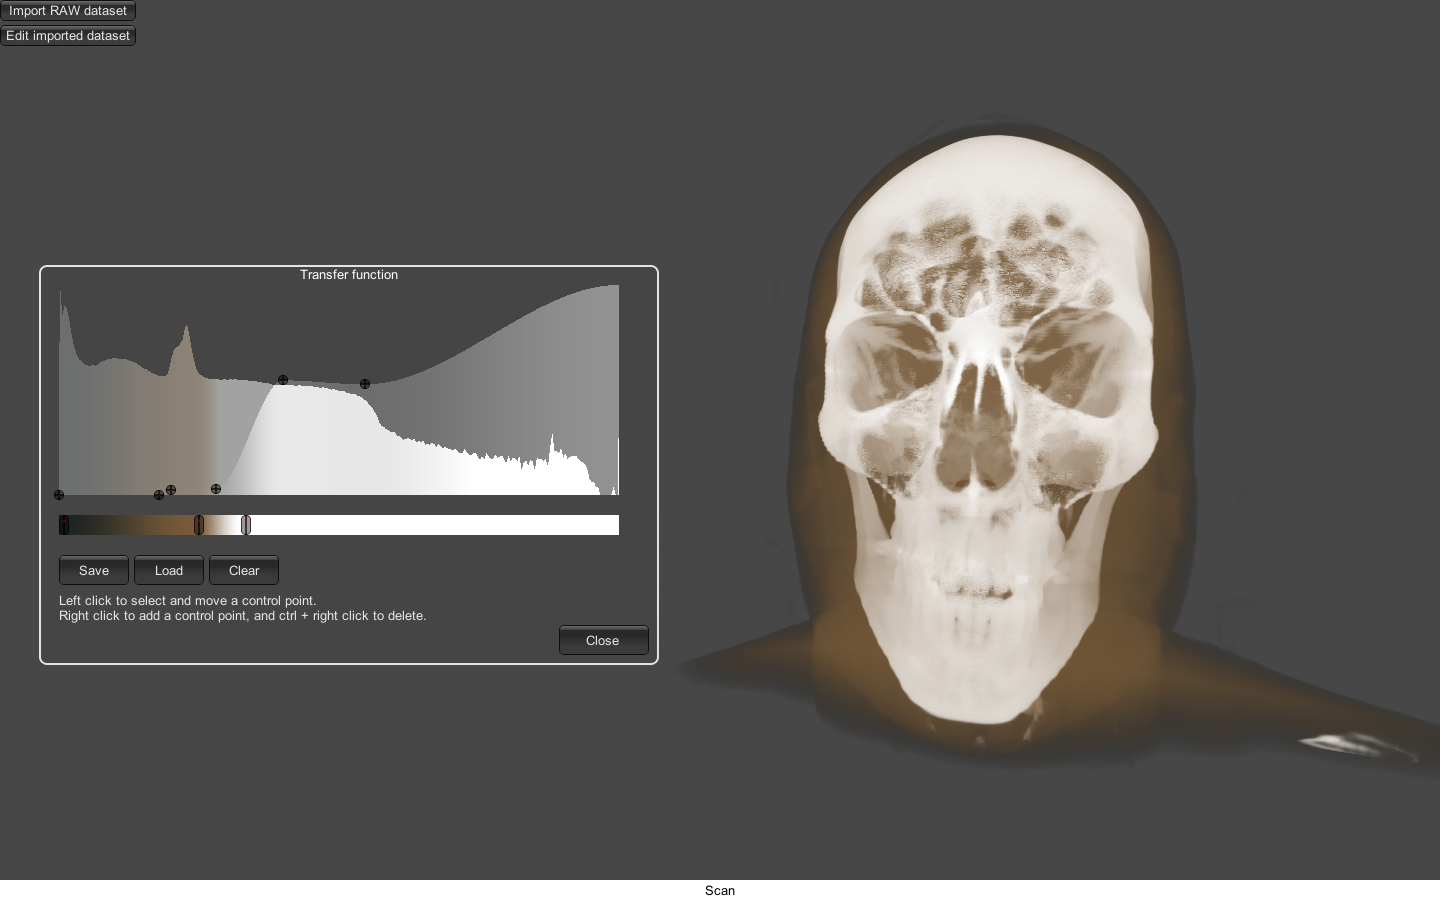
\includegraphics[width=0.7\textwidth]{KopfTransferfunktion}
%        \includegraphics[width=0.5\textwidth]{airplanes}
        
%        %\hspace*{0.25cm}
%        %\includegraphics[width=0.45\textwidth]{vorgang}
%        %\caption{Visualisierung eines Raytracing-Vorgangs \cite{Suffern}}
    \end{figure}

\end{block}


\end{column} % End of the second column



\begin{column}{.025\textwidth}\end{column} % Empty spacer column

\begin{column}{.465\textwidth}


\begin{block}{Unterschenkel + Transferfunktion}
  
    \begin{figure}
    	\center
        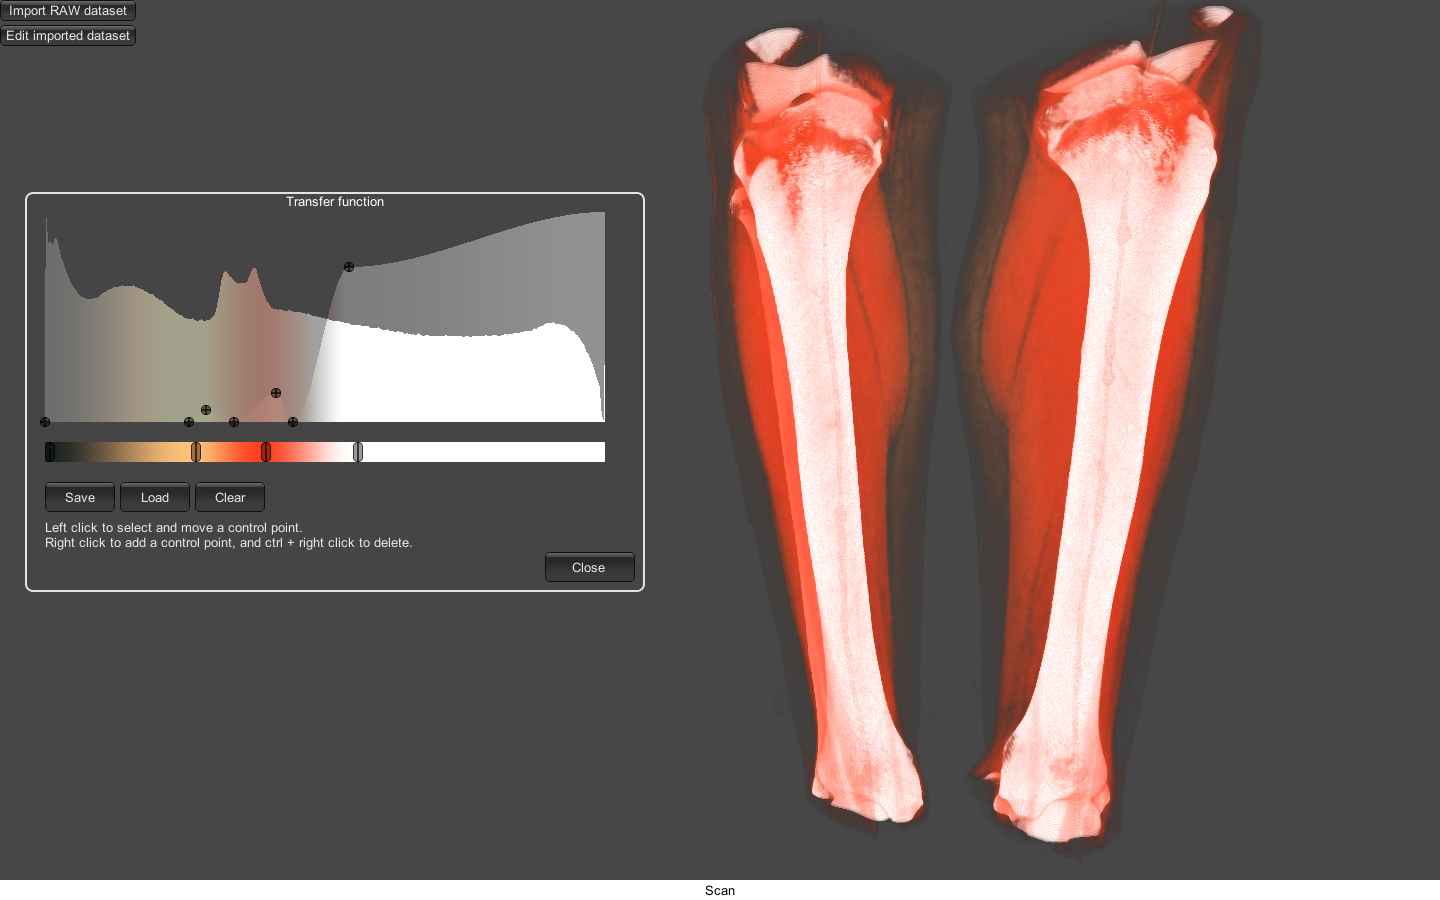
\includegraphics[width=0.7\textwidth]{KnieTransferfunktion}
%        \includegraphics[width=0.5\textwidth]{airplanes}
        
%        %\hspace*{0.25cm}
%        %\includegraphics[width=0.45\textwidth]{vorgang}
%        %\caption{Visualisierung eines Raytracing-Vorgangs \cite{Suffern}}
    \end{figure}
   
     
   
   
\end{block}


\end{column} % End of the second column



\begin{column}{.025\textwidth}\end{column} % Empty spacer column

\end{columns} % End of all the columns in the poster


\begin{columns}[t] % The whole poster consists of two major columns, each of which can be subdivided further with another \begin{columns} block - the [t] argument aligns each column's content to the top

\begin{column}{.025\textwidth}\end{column} % Empty spacer column

\begin{column}{.465\textwidth} % The first column


\begin{block}{Einstellungen}

    \newcommand{\imgheight}{127mm}
    \begin{figure}
    	\center
        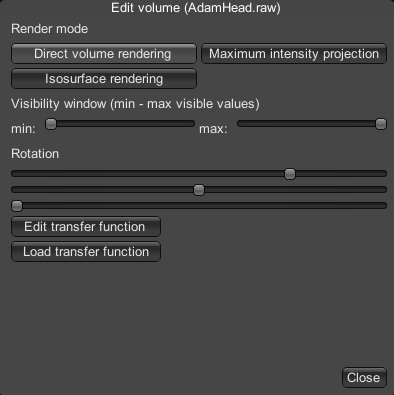
\includegraphics[height=\imgheight]{editMenu}
        \includegraphics[height=\imgheight]{transferfunction}
    \end{figure}


\end{block}

%\vspace{0.1cm}

\end{column} % End of the second column



\begin{column}{.025\textwidth}\end{column} % Empty spacer column

\begin{column}{.465\textwidth}

\begin{block}{Schnittebenen}

   \begin{figure}
       %\includegraphics[width=0.95\linewidth]{dxrWorkspace} %\textwidth]{dxrWorkspace}
       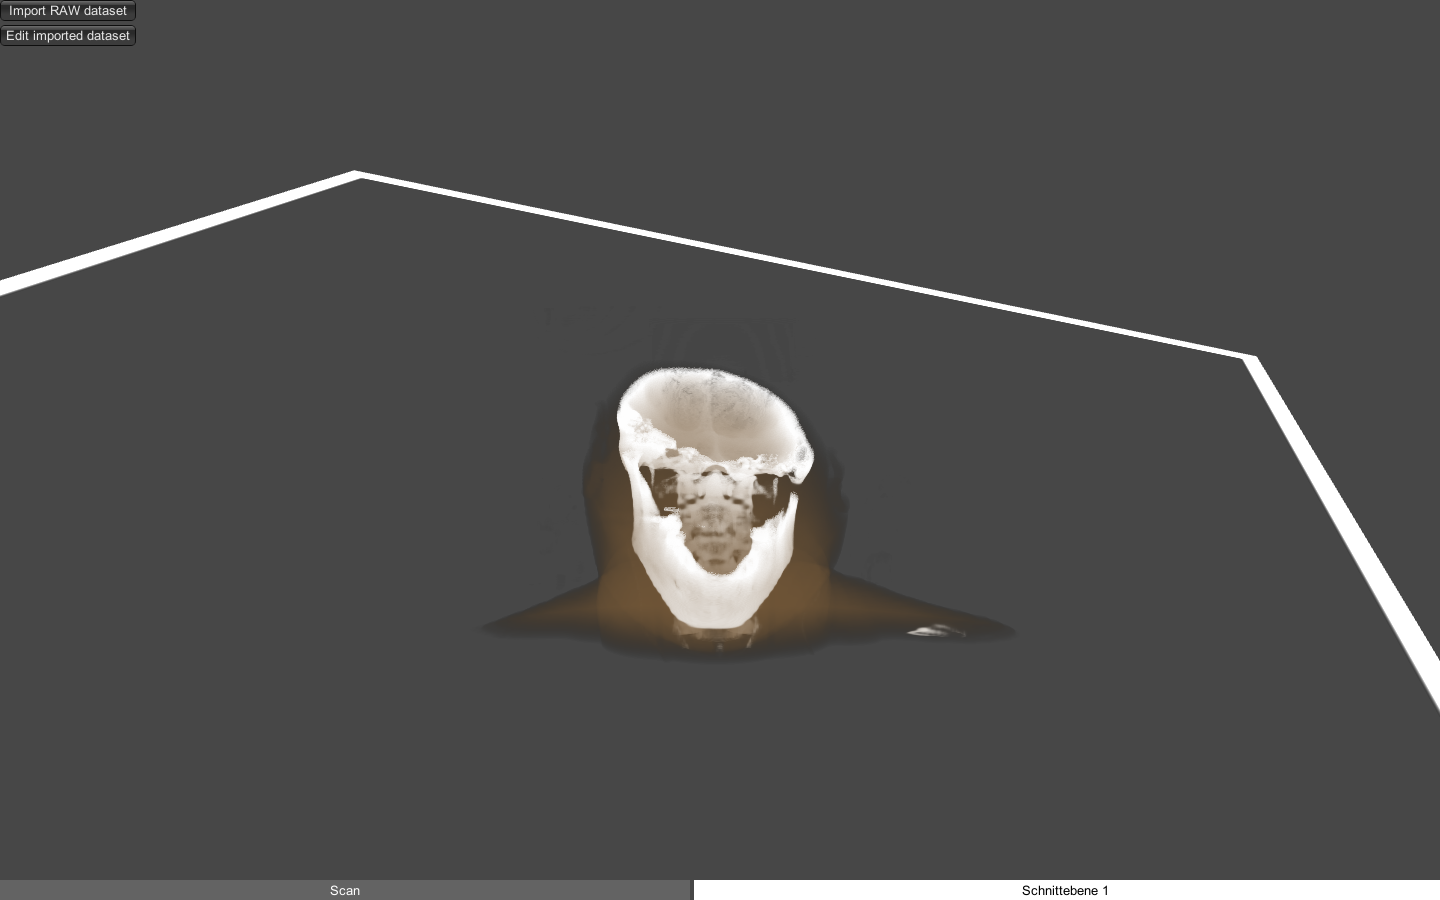
\includegraphics[width=0.325\textwidth]{slide01}
       \vspace{10px}
       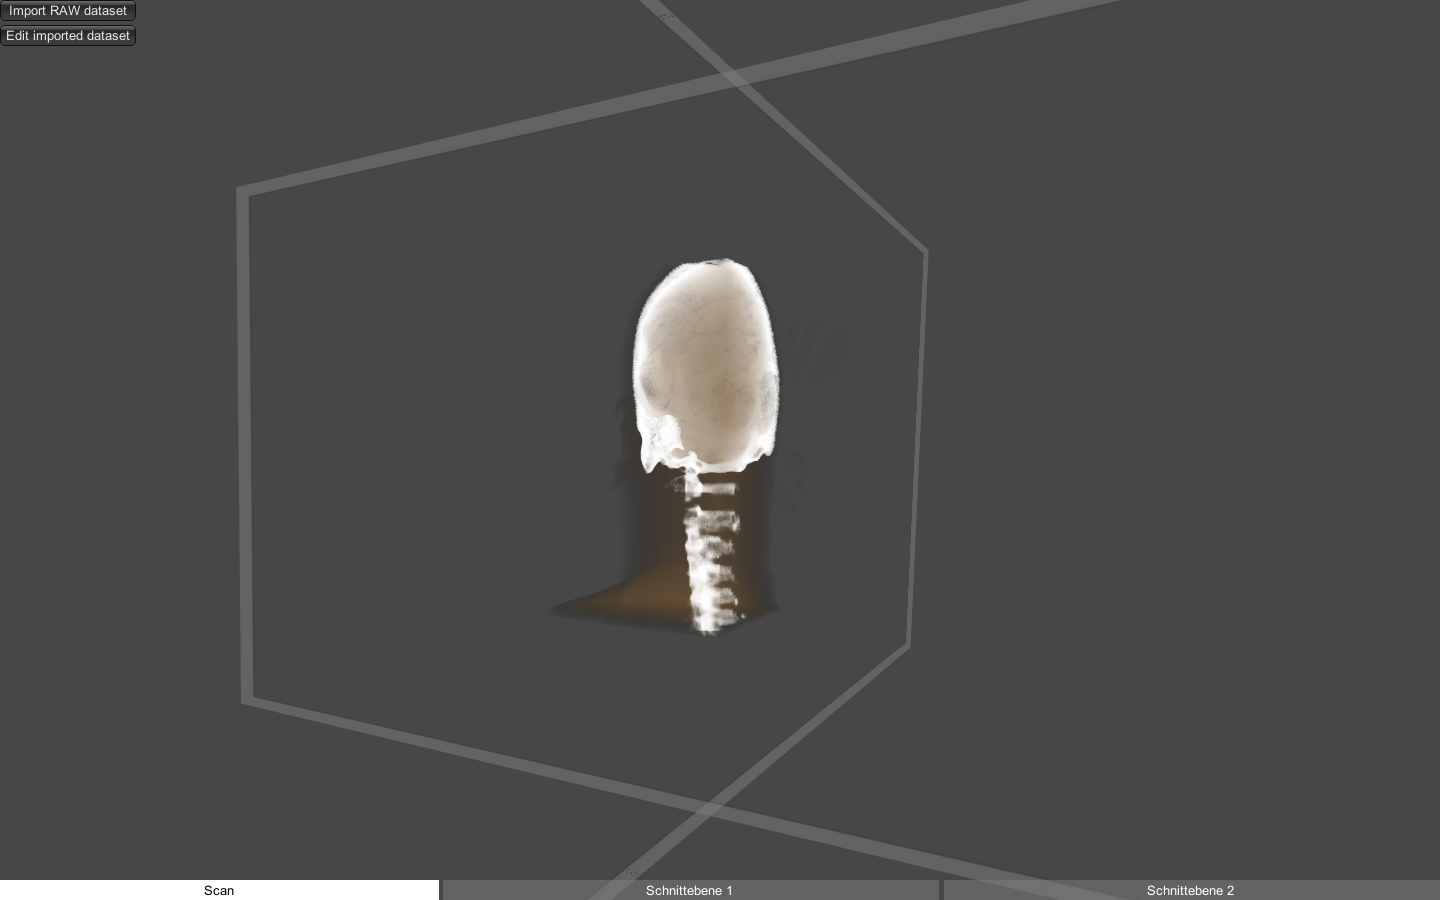
\includegraphics[width=0.325\textwidth]{slide02}
       \vspace{10px}
       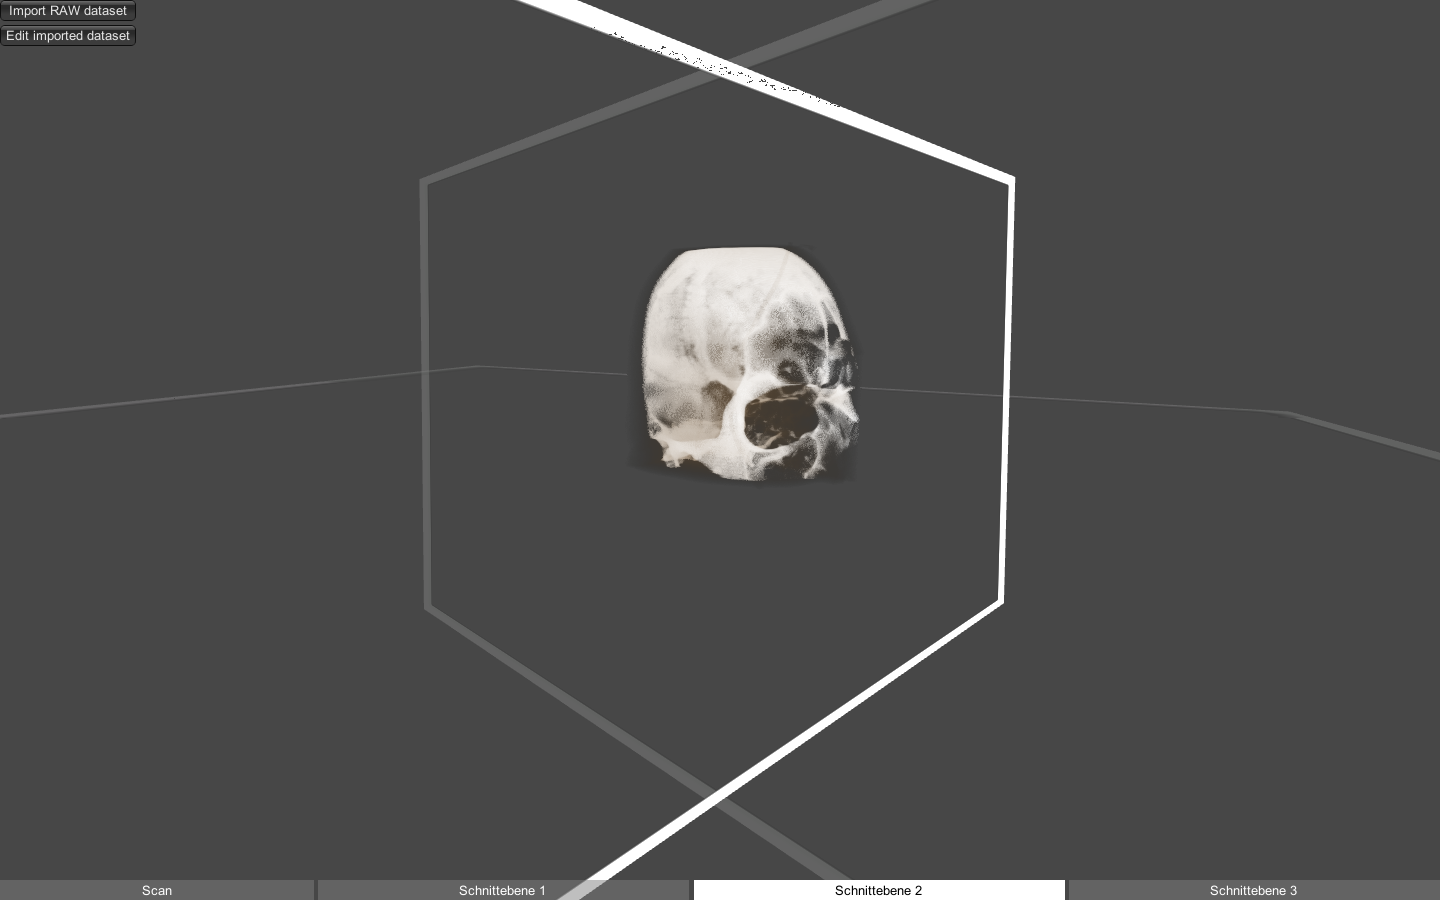
\includegraphics[width=0.325\textwidth]{slide03}
%       %\includegraphics[height=13.5cm]{hmd}
%   	  %\includegraphics[height=13.5cm]{CAVE_Crayoland}
   \end{figure}
%   
%   \vspace{10px}
%   
%   Weitere Informationen und Operationen sind in der Szene an den Wänden des Raumes positioniert. Jede Wand nimmt einen Kontext an, mit dem der Benutzer interagieren kann.
%   
%   
%   \vspace{10px}
%   
   \begin{itemize}
   \item bis zu acht Schnittebenen
   \item frei im Raum plazierbar
   \end{itemize}
   
     
   
   
\end{block}


\end{column} % End of the second column



\begin{column}{.025\textwidth}\end{column} % Empty spacer column

\end{columns} % End of all the columns in the poster


\begin{columns}[t] % The whole poster consists of two major columns, each of which can be subdivided further with another \begin{columns} block - the [t] argument aligns each column's content to the top

\begin{column}{.025\textwidth}\end{column} % Empty spacer column

\begin{column}{.465\textwidth} % The first column


\begin{block}{Kontakt}
\begin{columns}[t]
\begin{column}{.4\textwidth}
\begin{figure}[h]
% \vspace*{-1.0cm}
\centering

\includegraphics[width=.9\textwidth]{qrcode}
\vspace*{9mm}
\end{figure}
\end{column}



\begin{column}{.6\textwidth}
\vspace*{3.0cm}
\begin{itemize}[leftmargin=0pt]
    \item[] \Letter\ \href{rafaelhoock@gmail.com}{rafaelhoock@gmail.com}
    \item[] \Letter\ \href{manfred.brill@hs-kl.de}{manfred.brill@hs-kl.de}
    \item[] 
\includegraphics[scale=0.55]{github-mark} \href{https://github.com/VRLAB-HSKL/VirtualRadiologyPluraView}{github.com/VRLAB-HSKL/VirtualRadiologyPluraView}
\end{itemize}
\end{column}
\end{columns}

\end{block}

\end{column} % End of the second column

\begin{column}{.025\textwidth}\end{column} % Empty spacer column

\begin{column}{.465\textwidth}
\nocite{*} % Alles zitieren in sample.bib
\begin{block}{Literatur}
 \bibliographystyle{eg-alpha-doi}
 \bibliography{sample}
\end{block}

% \begin{block}{Literatur}

% \begin{itemize}

% \item Ref01
% \item Ref02

% \end{itemize}


% \end{block}

\end{column}

\begin{column}{.025\textwidth}\end{column} % Empty spacer column

\end{columns} % End of all the columns in the poster



%----------------------------------------------------------------------------------------








\end{frame} % End of the enclosing frame

\end{document} 